\documentclass[11pt]{article}

\usepackage[T1]{fontenc}
\usepackage[utf8]{inputenc}
\usepackage[brazilian]{babel}
\usepackage[margin=1in]{geometry}
\usepackage{booktabs}
\usepackage{graphicx}
\usepackage{xcolor}
\usepackage{amsmath}
\usepackage{microtype}
\usepackage[hidelinks]{hyperref}

\title{\textbf{Dois Desertos: Acesso Hospitalar no Brasil sob\\
Distância e sob Fluxo Revelado}}
\author{Darcio Genicolo-Martins\thanks{Insper. Relatório técnico descritivo;
identificação causal de efeitos de acesso é desenvolvida em trabalho relacionado
e não é reivindicada aqui. Código e pipeline reprodutível acompanham o relatório.}}
\date{\today}

\begin{document}
\maketitle

\begin{abstract}
\noindent
Políticas de acesso hospitalar são desenhadas sobre mapas de distância, mas os
pacientes viajam para onde há cuidado, não para o ponto mais próximo. Este
relatório descritivo confronta, para os 5.492 municípios brasileiros (2015--2022),
o deserto de distância (km ao hospital ativo mais próximo) com o deserto de
fluxo (burden efetivo de viagem, ponderado por onde os residentes de fato
internam, a partir de 94 milhões de internações do SIH). As duas medidas
correlacionam-se apenas moderadamente ($r=0{,}55$), e dos municípios sinalizados
como deserto por algum dos conceitos, 60\% o são por apenas um. O resultado
central: 595 municípios, com cerca de 9,2 milhões de habitantes, têm hospital
próximo no mapa mas são desertos de fluxo --- invisíveis a uma política de
distância --- e recaem desproporcionalmente sobre municípios pobres e dependentes
do SUS. Um overlay com mortalidade evitável mostra por que a associação simples
engana e por que a pergunta causal exige outro desenho. Medir acesso por
quilômetros não é uma aproximação inócua: é um mapa diferente, que erra de forma
sistemática e identificável.

\medskip
\noindent\textbf{Palavras-chave:} acesso hospitalar, desertos de saúde, fluxo de
pacientes, SUS, Brasil. \quad\textbf{JEL:} I11, I14, I18, R12.
\end{abstract}

% Secao 0 - Sumario executivo (1 pag). Quem le so isto entende o achado.
% Headline number unico, repetido no abstract e na conclusao.

\section*{Sumário executivo}
\addcontentsline{toc}{section}{Sumário executivo}

\noindent\textbf{Tese.} Desertos hospitalares medidos em quilômetros e desertos
medidos pelo fluxo real de pacientes não são o mesmo mapa --- e o gap entre eles
identifica os municípios que uma política de acesso baseada em distância
sistematicamente não enxerga.

\medskip
\noindent\textbf{O que fazemos.} Para os 5.492 municípios brasileiros (2015--2022),
confrontamos o deserto de \emph{distância} (km ao hospital ativo mais próximo)
com o deserto de \emph{fluxo} (burden efetivo de viagem, ponderado por onde os
pacientes de fato internam, construído de 94 milhões de internações do SIH). O
exercício é descritivo; nenhuma reivindicação causal é feita.

\medskip
\noindent\textbf{Três números que o relatório sustenta.}
\begin{itemize}
\item As duas medidas correlacionam-se apenas moderadamente ($r=0{,}55$): a
  distância ao hospital mais próximo explica cerca de 30\% da variação no burden
  efetivo de fluxo. O paciente típico viaja 32~km \emph{além} do hospital mais
  próximo.
\item Dos municípios sinalizados como deserto por qualquer dos dois conceitos,
  60\% o são por apenas um deles. Os mapas discordam sobre a maioria dos
  desertos.
\item \textbf{595 municípios, onde vivem cerca de 9,2 milhões de pessoas, têm um
  hospital por perto no mapa mas são desertos de fluxo} --- seus pacientes
  viajam, em média efetiva, 91~km, e 90\% das internações deixam o município.
  São invisíveis a uma política de distância.
\item O deserto de fluxo tem dois lados. Os mesmos municípios que perdem
  pacientes têm uma vez e meia menos médicos por habitante e menos especialistas
  --- apesar de terem leito ---, e sangram médicos ano após ano para os centros
  que absorvem seus pacientes. A ausência do cuidado e a de quem o presta
  caminham juntas.
\end{itemize}

\medskip
\noindent\textbf{A figura-síntese.} A Figura~\ref{fig:divergencia} pinta o
desacordo: em vermelho, os desertos de fluxo ocultos à distância, no interior do
Nordeste e do Centro-Oeste; em azul, onde a distância exagera o isolamento, na
Amazônia de viagem fluvial. Os perfis confirmam que o ponto cego recai sobre
municípios mais pobres e dependentes do SUS, e que ter um hospital local não
equivale a ter o cuidado de que se precisa --- o lado da oferta confirma por quê:
esses municípios têm menos médicos, menos especialistas e perdem médicos para os
mesmos hubs (Figura~\ref{fig:redes_medicas}). A pergunta sobre o custo em saúde
do isolamento exige um desenho causal e fica reservada a trabalho relacionado;
este relatório entrega a medida e a geografia.


% Secao 1 - Motivacao e o gancho. Abre com a tensao economica, nao com o SUS.

\section{Motivação: dois mapas para o mesmo país}
\label{sec:motivacao}

Políticas de acesso à saúde são desenhadas sobre mapas. Programas de combate a
desertos de maternidade, a regionalização do SUS em regiões de saúde, a alocação
de novos leitos --- todos perguntam, no fundo, a mesma coisa: quão longe está o
hospital mais próximo? A distância é a régua natural porque é observável,
barata e intuitiva. O problema é que o paciente não viaja em linha reta ao ponto
mais próximo. Ele viaja para onde há o cuidado de que precisa, e esse destino
revelado frequentemente contradiz o mapa.

Este relatório leva essa contradição a sério. Ele contrasta dois conceitos de
deserto hospitalar para os \valNmunic{} municípios brasileiros entre 2015 e 2022. O
primeiro é o deserto de \emph{distância}: a quilometragem ao hospital ativo mais
próximo, a medida que a política baseada em mapa enxerga. O segundo é o deserto
de \emph{fluxo}: o burden efetivo de viagem, ponderado pelos hospitais em que os
residentes de fato internam. Os dois compartilham o suficiente para medir o
mesmo fenômeno e divergem o suficiente para que a escolha da régua mude quem é
classificado como desassistido.

A pergunta é deliberadamente descritiva, não causal: \emph{onde, e para quem, os
dois conceitos discordam?} A divergência não é pequena nem aleatória. Existe um
contingente grande de municípios que o mapa de distância declara atendidos ---
têm um hospital por perto --- mas cujos pacientes, na prática, viajam longe
porque o hospital local não resolve o que precisam. Há também o inverso, na
Amazônia, onde a distância rodoviária exagera um isolamento que o fluxo real, por
rio e local, desmente. Medir acesso por quilômetros, mostramos, não é uma
aproximação inócua: é um mapa diferente, que erra de forma sistemática e
identificável. A questão de se essa diferença custa vidas é real, mas exige
identificação causal e fica explicitamente fora do escopo deste relatório
(Seção~\ref{sec:mortalidade}); aqui, estabelecemos a medida e a geografia do
desacordo.

% Secao 3 - Dados e construcao. Reaproveita convencoes do paper18.
% Disciplina: descritivo. Numeros com % src.

\section{Dados e construção}
\label{sec:dados}

O relatório combina quatro fontes para o período 2015--2022, todas no nível do
município de residência. Os fluxos de pacientes vêm do Sistema de Informações
Hospitalares (SIH/DATASUS): cada Autorização de Internação Hospitalar (AIH)
registra o município de residência do paciente e o estabelecimento (CNES) onde a
internação ocorreu, o que permite construir o grafo bipartido
residência~$\rightarrow$~hospital que define o fluxo. O universo de hospitais
ativos por ano vem do Cadastro Nacional de Estabelecimentos de Saúde (CNES),
restrito a estabelecimentos com leito hospitalar instalado. As distâncias e os
tempos de viagem usam os centroides municipais do IBGE e a malha rodoviária via
OSRM. A população, denominador das taxas, vem das estimativas IBGE/SIDRA.

Duas disciplinas de construção merecem registro. A primeira é o \emph{firewall}
entre residência e provedor: toda exposição é atribuída pelo município onde o
paciente \emph{mora}, nunca pelo município onde o hospital opera, de modo que o
fluxo mede a dependência revelada do morador, não a atividade do hospital. A
segunda são as armadilhas conhecidas do SIH: contamos AIH de internação (AIH-1)
e não as de continuação (AIH-5), para não duplicar episódios, e tratamos o SIH
como retrato do SUS --- internações na saúde suplementar não aparecem, o que
subestima a oferta efetiva em municípios de alta penetração privada, ressalva
que a Seção~\ref{sec:divergencia} incorpora via cobertura ANS.

A amostra cobre 5.588 municípios de residência, 10.450 hospitais com leito ativos
na janela e 94,0 milhões de internações.% src: bloco cobertura - n_mun_res 5588, n_hosp_beds 10450, n_aih 93.996.098
O recorte analítico do relatório usa os 5.492 municípios com fluxo suficiente
para um burden efetivo bem definido.% src: master_muni_panel N=5492 (apos filtro NaN travel_burden)

% Secao 4 - O deserto de distancia (descritivo).

\section{O deserto de distância}
\label{sec:distancia}

A medida que uma política de acesso baseada em mapa adota é direta: a distância
do município ao hospital ativo mais próximo. A Figura~\ref{fig:distance_map} a
traça para o Brasil. A mediana é de 16~km e, para metade dos municípios, o
hospital mais próximo está a menos de meia hora de estrada; só no quartil
superior a distância passa de 27~km, e apenas 5\% dos municípios estão a mais de
62~km.% src: distribuicao iso_km - p50 16, p75 27, p95 62, max 378
Lido isoladamente, o mapa de distância é tranquilizador: a maior parte do país
aparece em tons escuros, ``perto''.

A exceção visível é a Amazônia, onde a distância ao hospital mais próximo chega a
centenas de quilômetros. Mas é justamente ali que a medida é mais frágil. A
distância rodoviária pressupõe que o deslocamento se dá por estrada; no Norte,
ele se dá por rio, e a quilometragem sobre a malha viária superestima --- ou
simplesmente não representa --- a viagem real. O mapa de distância, portanto,
erra em dois sentidos que só ficarão visíveis quando confrontado com o fluxo:
exagera o isolamento onde o rio supre a estrada e o subestima onde o hospital
próximo não é o hospital usado.

% Figura 3 - choropleth do deserto de distancia. src: 12_fig_desert_maps.py
\begin{figure}[t]
\centering
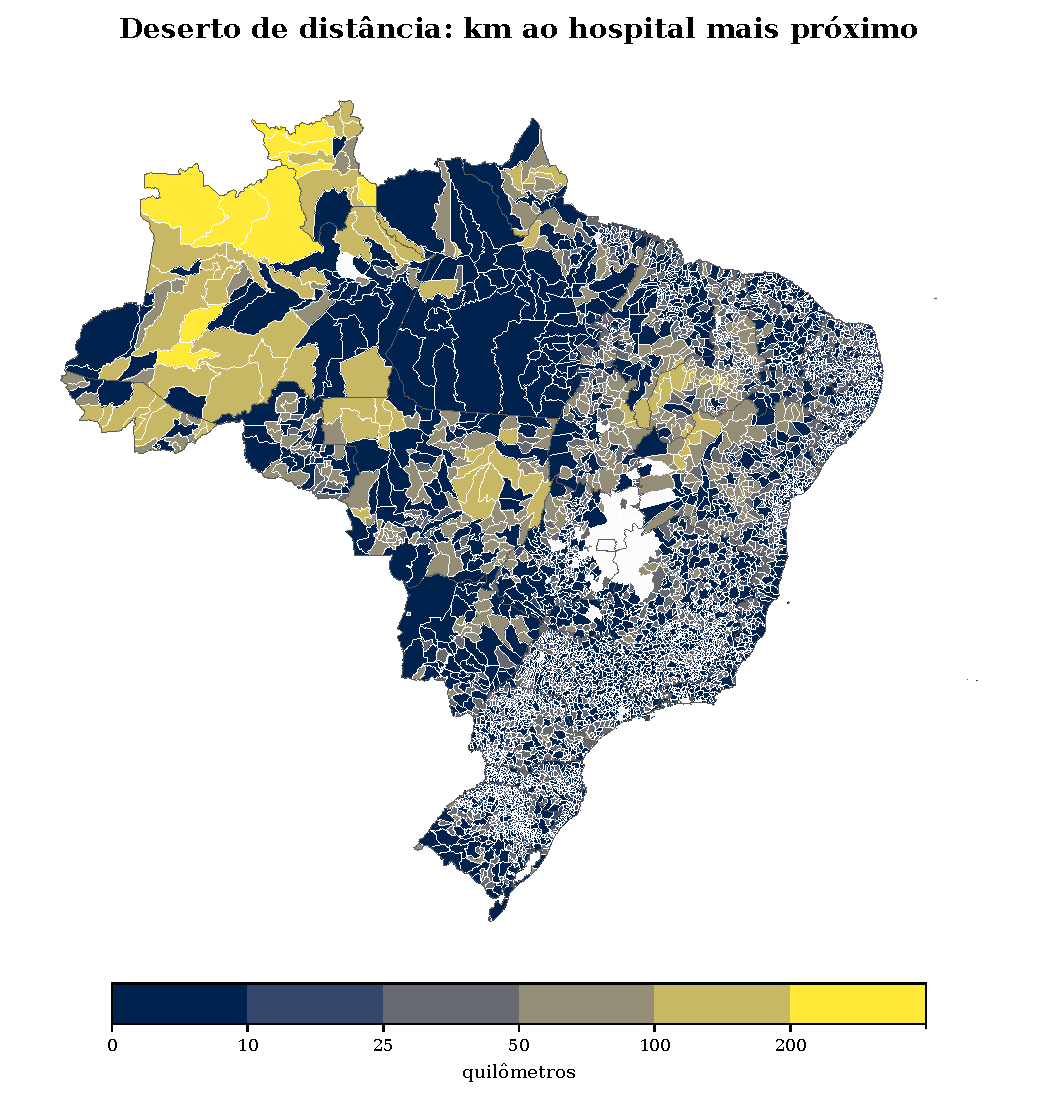
\includegraphics[width=0.86\linewidth]{../04_figures/fig3_distance_map.pdf}
\caption{\textbf{Deserto de distância: quilômetros ao hospital ativo mais
próximo.} Cada município colorido pela distância de centroide ao hospital com
leito mais próximo, 2015--2022. A escala de cores (em km) é idêntica à da
Figura~\ref{fig:flow_map}, permitindo comparação direta. A maior parte do país
aparece em tons escuros (perto); o isolamento de distância concentra-se na
Amazônia, onde, contudo, a malha rodoviária não representa o deslocamento real
por rio. Projeção Brasil Polyconic (EPSG:5880). Fonte: CNES, OSRM, IBGE.}
\label{fig:distance_map}
\end{figure}

% Secao 5 - O deserto de fluxo (descritivo). Medida primaria F1.

\section{O deserto de fluxo}
\label{sec:fluxo}

O deserto de fluxo substitui ``qual o hospital mais próximo'' por ``a que
distância está o cuidado que o paciente de fato usa''. A medida primária é o
burden efetivo de fluxo F1: a distância de viagem ponderada pelo número de
internações em cada destino, de modo que um município cujos pacientes se espalham
por hubs distantes acumula burden alto mesmo que tenha um hospital ao lado.
Formalmente, para o município $m$,
\[
F1_m \;=\; \frac{\sum_h n_{m,h}\, d\big(m, \text{mun}(h)\big)}{\sum_h n_{m,h}},
\]
onde $n_{m,h}$ é o número de internações de residentes de $m$ no hospital $h$ e
$d(\cdot)$ a distância entre centroides. Operacionalizações alternativas ---
isolamento em uma rede de co-paciência (embeddings) e concentração dos destinos
(HHI) --- concordam com F1 e são tratadas como robustez no apêndice.

A Figura~\ref{fig:flow_map} mostra F1 na mesma escala de quilômetros da
Figura~\ref{fig:distance_map}, e o contraste é o ponto central do relatório. O
burden efetivo mediano é de 49~km --- mais do triplo da distância mediana ao
hospital mais próximo --- e 5\% dos municípios superam 136~km.% src: distribuicao f1_km - p50 49, p75 73, p95 136, max 619
Na mesma paleta, o mapa de fluxo é visivelmente mais quente: vastas áreas do
interior do Nordeste, do Centro-Oeste e do Norte que a distância pintava como
``perto'' carregam burden de viagem alto, porque o cuidado efetivamente usado
está longe. O deserto de fluxo não é um recorte do deserto de distância; é um
mapa próprio, e a Seção~\ref{sec:divergencia} mede exatamente onde os dois
divergem e quem mora na diferença.

% Figura 4 - choropleth do deserto de fluxo (F1). src: 12_fig_desert_maps.py
\begin{figure}[t]
\centering
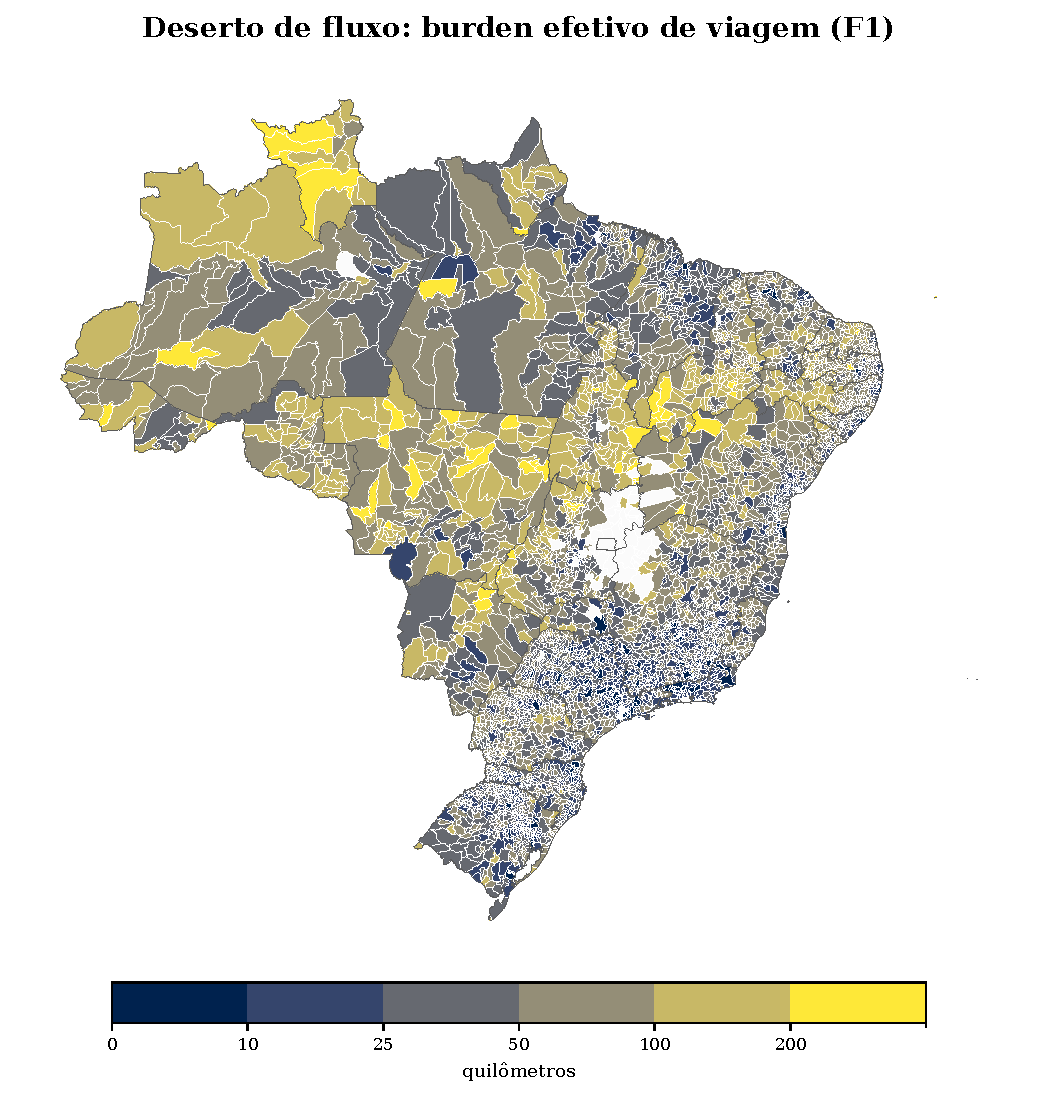
\includegraphics[width=0.86\linewidth]{../04_figures/fig4_flow_map.pdf}
\caption{\textbf{Deserto de fluxo: burden efetivo de viagem (F1).} Cada município
colorido pelo burden efetivo de fluxo --- distância de viagem ponderada por onde
os pacientes de fato internam ---, 2015--2022, na mesma escala de quilômetros da
Figura~\ref{fig:distance_map}. O mapa é visivelmente mais quente: o burden
efetivo mediano (\valMedFround~km) é o triplo da distância mediana ao hospital mais próximo,
e o interior do Nordeste, do Centro-Oeste e do Norte carrega burden alto onde a
distância sugeria proximidade. Projeção Brasil Polyconic (EPSG:5880). Fonte:
SIH/DATASUS, OSRM, IBGE.}
\label{fig:flow_map}
\end{figure}

% Secao 6 - o coracao do relatorio: concordancia e divergencia distancia x fluxo.
% Disciplina: descritivo, associativo. Numeros = macros de values.tex.

\section{Concordância e divergência entre os dois desertos}
\label{sec:divergencia}

As seções anteriores construíram duas medidas de deserto hospitalar: a distância
ao hospital ativo mais próximo, que uma política de acesso baseada em mapa
enxerga, e o burden efetivo de fluxo F1, que pondera a viagem por onde os
pacientes de fato internam. Se as duas dissessem a mesma coisa, F1 seria
redundante e este relatório, desnecessário. Mas não dizem: concordam o
suficiente para medir o mesmo fenômeno e divergem o suficiente para que a escolha
da medida mude quem é classificado como desassistido. Resta caracterizar onde, e
para quem, a divergência aparece.

\subsection{Quanto um conceito é redundante com o outro}

A Figura~\ref{fig:scatter} cruza as duas medidas no município. A correlação é
moderada: $r = \valCorrFD$, de modo que a distância ao hospital mais próximo
explica cerca de \valRtwoFD\% da variação no burden efetivo de fluxo.% src: 11_fig2_scatter; corr 0.551, R2 0.304
O que sobra não é ruído. Quase toda a massa de pontos está \emph{acima} da
diagonal $F1 = \text{distância}$: o paciente típico não interna no hospital mais
próximo, e o burden efetivo mediano (\valMedF~km) é o triplo da distância mediana
ao hospital mais próximo (\valMedIso~km), uma diferença mediana de \valMedGap~km
que mede o desvio revelado em relação ao mapa.% src: 01_build_f1_divergence headline
A consequência para mensuração é direta. Definindo deserto como o quartil
superior de cada medida, dos municípios sinalizados como deserto por
\emph{algum} dos dois conceitos, \valPctDisagree\% o são por apenas um deles; e
\valPctFlowMissed\% dos desertos de fluxo são invisíveis ao conceito de
distância.% src: bloco síntese - pct_disagree 60.5, pct_flow_missed 43.3
Trocar quilômetros por fluxo revelado não recalibra uma medida --- redesenha o
mapa de quem precisa de atenção.

\subsection{O mapa da divergência}

A Figura~\ref{fig:divergencia} pinta cada município pelo quadrante que ocupa, e
a geografia do desacordo não é aleatória. Os desertos de fluxo ocultos à
distância (vermelho) concentram-se no interior do Nordeste e do Centro-Oeste:
municípios com um hospital por perto no mapa, mas cuja necessidade de internação
escoa para hubs distantes. O padrão inverso (azul) domina a Amazônia, onde a
distância rodoviária ao hospital mais próximo é grande mas o fluxo efetivo é
curto --- reflexo de que a malha de estradas não representa o deslocamento real,
por rio, e de que o atendimento, quando ocorre, ocorre localmente. O deserto
pleno, em que os dois conceitos concordam, ocupa o Norte mais remoto; a
concordância de que não há deserto cobre o Sul e o Sudeste populosos.

\subsection{Quem vive em cada quadrante}

A Tabela~\ref{tab:perfis} traça o perfil dos quadrantes e revela três padrões.
O primeiro desfaz o paradoxo aparente do quadrante perto-mas-isolado: longe de
não terem oferta, esses municípios têm a \emph{maior} presença de hospital local
da tabela (\valFOhosp\% têm ao menos um leito hospitalar instalado) e ainda assim
90\% de suas internações saem do município.% src: profiles_by_quadrant.csv
O hospital local existe, mas resolve pouco; a necessidade real --- a que exige
complexidade --- viaja. É exatamente o tipo de isolamento que a contagem de
leitos no mapa não captura e o fluxo revela.

O segundo padrão é distributivo. Os três quadrantes de deserto são
sistematicamente mais pobres (PIB per capita em torno de R\$~13--14~mil) do que o
quadrante conectado (R\$~22~mil), de modo que a fricção de acesso, medida por
qualquer dos conceitos, recai sobre os municípios de menor renda. O terceiro
padrão qualifica o papel do setor privado: a cobertura de saúde suplementar é
baixa nos desertos (\valBOans\% a \valDOans\%) e bem maior no quadrante conectado
(\valNEans\%). Onde o fluxo revela isolamento, não há rede privada que absorva a
demanda --- o gap morde com força em municípios dependentes do SUS. (A relação
dos quadrantes com mortalidade evitável é deliberadamente adiada para a
Seção~\ref{sec:mortalidade}, que mostra por que a associação simples engana.)

\begin{table}[t]
\centering
\caption{Perfil dos quadrantes distância $\times$ fluxo}
\label{tab:perfis}
\footnotesize
\begin{tabular}{lrrrrrrr}
\toprule
Quadrante & Munic. & Pop. & Dist. & F1 & Fluxo que & Hosp. & PIB pc \\
          &        & (mi) & (km)  & (km) & sai      & local & (R\$ mil) \\
\midrule
Perto, deserto em fluxo & \valFOn & \valFOpop  & \valFOiso & \valFOf  & \valFOout & \valFOhosp\% & \valFOpib \\
Deserto pleno           & \valBOn & \valBOpop  & \valBOiso & \valBOf  & \valBOout & \valBOhosp\% & \valBOpib \\
Longe, conectado        & \valDOn & \valDOpop  & \valDOiso & \valDOf  & \valDOout & \valDOhosp\% & \valDOpib \\
Sem deserto             & \valNEn & \valNEpop  & \valNEiso & \valNEf  & \valNEout & \valNEhosp\% & \valNEpib \\
\bottomrule
\end{tabular}
\par\smallskip
\begin{minipage}{0.92\linewidth}
\footnotesize
\textit{Nota:} Medianas municipais, exceto N e população (soma). ``Fluxo que
sai'' $=$ fração das internações em hospital fora do município. ``Hosp.\ local''
$=$ \% de municípios com ao menos um leito hospitalar instalado e ativo na
janela. Cobertura privada (ANS) mediana, omitida da tabela por brevidade:
\valFOans\%, \valBOans\%, \valDOans\% e \valNEans\%, na ordem das linhas. Fonte:
SIH/DATASUS, CNES, IBGE, ANS.
\end{minipage}
\end{table}

\subsection{Quatro municípios, por inspeção}

Os quadrantes ganham concretude em casos individuais. \textbf{Fonte Boa (AM)}
está a \valFonteBoaIso~km do hospital mais próximo pela malha rodoviária, mas
\valFonteBoaLocal\% de suas internações ocorrem localmente e seu burden efetivo é
de apenas \valFonteBoaF~km: o mapa o declara deserto profundo; o fluxo, não.
\textbf{Soledade (PB)} é o espelho: o hospital mais próximo está a
\valSoledadeIso~km, mas \valSoledadeOut\% dos pacientes saem e viajam, em média
efetiva, \valSoledadeF~km --- um deserto de fluxo que a distância classifica como
atendido. \textbf{Anchieta (SC)} leva o ponto ao extremo: \emph{sedia} um
hospital (distância zero) e, ainda assim, todas as suas internações deixam o
município; ter um leito não é ter o cuidado de que se precisa.% src: casos canônicos
No contraponto, \textbf{Sobral (CE)} --- polo regional do interior --- retém
seus pacientes (apenas \valSobralOut\% saem, burden de \valSobralF~km) apesar de
não ser capital: estar no interior não é, por si, ser deserto, desde que o
município seja um hub de fato. A distinção que separa Soledade de Sobral não
aparece em quilômetros; aparece no fluxo.

% Figure 1 - mapa da divergencia distancia x fluxo.
% Gerada por 03_analysis/10_fig1_divergence_map.py (% src).
% Caption autoexplicativa: funciona destacada do paper (teste do editor cansado).

\begin{figure}[t]
\centering
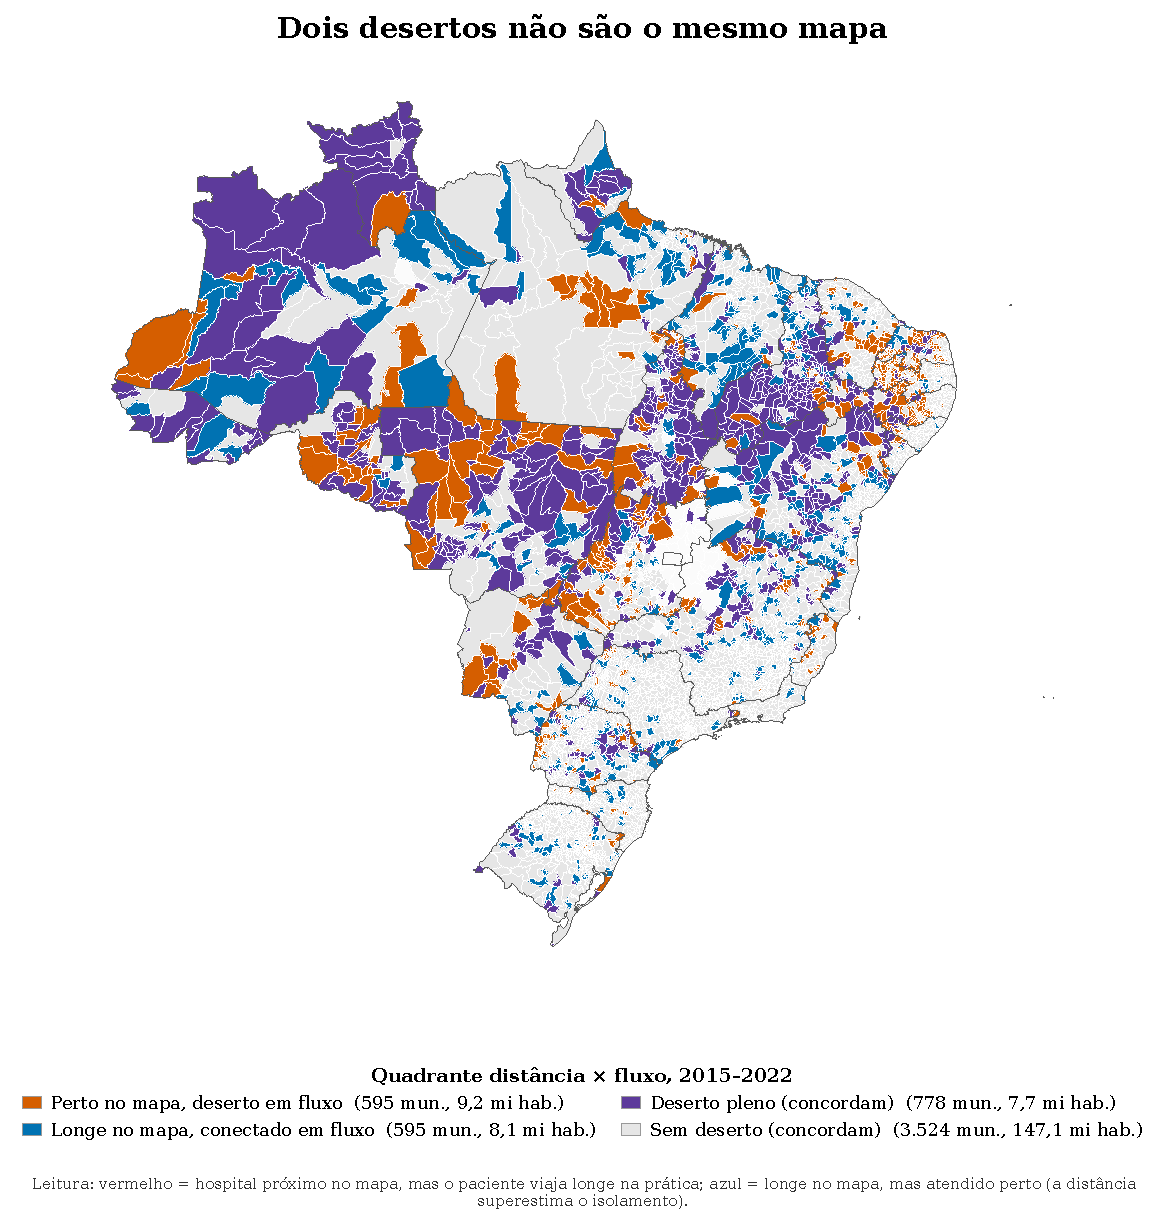
\includegraphics[width=0.9\linewidth]{../04_figures/fig1_divergence_map.pdf}
\caption{\textbf{Desertos de distância e desertos de fluxo não são o mesmo mapa.}
Cada município brasileiro pintado pelo quadrante que ocupa quando se cruza o
deserto de \emph{distância} (quilômetros ao hospital ativo mais próximo) com o
deserto de \emph{fluxo} (F1, burden efetivo de viagem ponderado por onde os
pacientes de fato internam), 2015--2022. Deserto $=$ acima do quartil superior
de cada medida. Os dois quadrantes de desacordo são o objeto do relatório: em
\textcolor[HTML]{D55E00}{\textbf{vermelho}}, os 595 municípios
(\textasciitilde9,2 milhões de habitantes) com hospital próximo no mapa mas cujos
pacientes viajam longe na prática --- o ponto cego de uma política de acesso
baseada em distância; em \textcolor[HTML]{0072B2}{\textbf{azul}}, os 595 onde a
distância no mapa superestima o isolamento porque o atendimento efetivo é
próximo, padrão concentrado na Amazônia, onde a malha rodoviária não representa o
deslocamento real. Em \textcolor[HTML]{5D3A9B}{\textbf{roxo}}, desertos pelos
dois conceitos; em cinza, municípios em que os conceitos concordam que não há
deserto. Projeção Brasil Polyconic (SIRGAS 2000, EPSG:5880); fronteiras
estaduais em cinza. Fonte: SIH/DATASUS (fluxos), malha municipal IBGE 2010,
matriz de distância OSRM.}
\label{fig:divergencia}
\end{figure}

% Figure 2 - scatter F1 x distancia (Secao 6.1).
% Gerada por 03_analysis/11_fig2_scatter_flow_distance.py.

\begin{figure}[t]
\centering
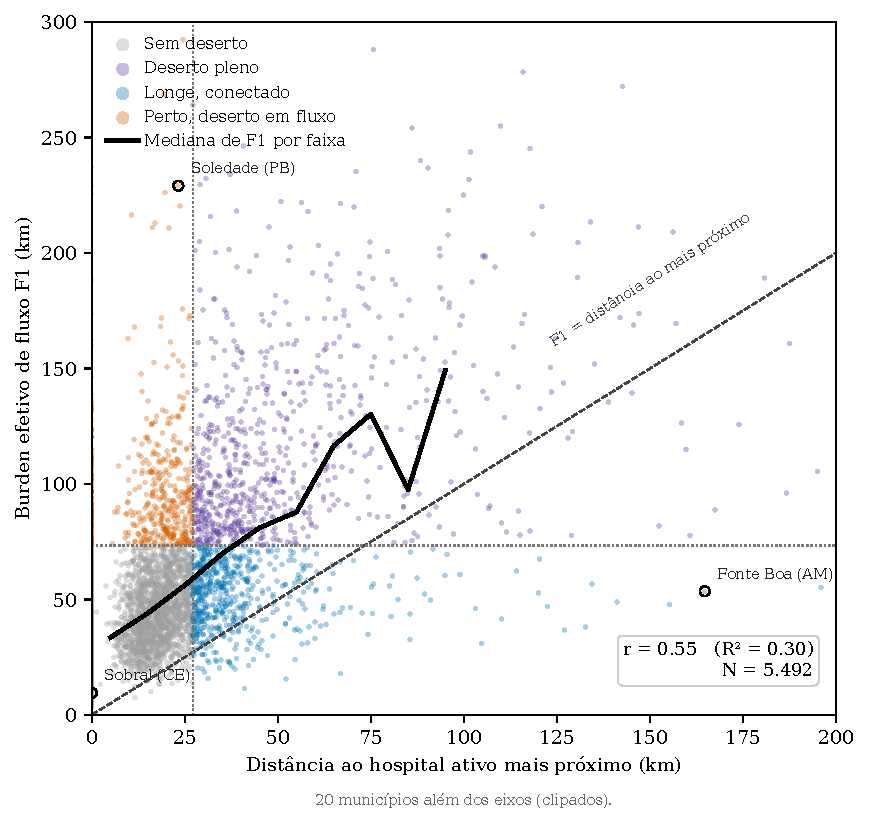
\includegraphics[width=0.82\linewidth]{../04_figures/fig2_scatter.pdf}
\caption{\textbf{Fluxo e distância são correlacionados, mas não intercambiáveis.}
Cada ponto é um município ($N=5.492$): no eixo horizontal, a distância ao
hospital ativo mais próximo; no vertical, o burden efetivo de fluxo F1.
A correlação é moderada ($r=0{,}55$, $R^2=0{,}30$). Quase toda a massa está acima
da diagonal $F1=\text{distância}$ (tracejada), indicando que os pacientes
internam além do hospital mais próximo. Cores marcam os quadrantes da
Tabela~\ref{tab:perfis}; linhas pontilhadas são os cortes de deserto (quartil
superior de cada medida). A curva preta é a mediana de F1 por faixa de distância.
Âncoras: Soledade (PB), perto no mapa mas deserto em fluxo; Fonte Boa (AM), longe
mas conectado; Sobral (CE), polo do interior sem deserto. Fonte: SIH/DATASUS,
OSRM, IBGE.}
\label{fig:scatter}
\end{figure}

% Seção 8 — Overlay descritivo com mortalidade evitável.
% Enquadramento: CAUTELA DE MENSURAÇÃO, não "desertos matam".
% Disciplina: estritamente associativo. O causal mora no paper18.
% Números rastreados a 03_analysis/04_build_age_std_mortality.py e
% mortality_crude_vs_agestd_by_quadrant.csv (% src: ... abaixo).

\section{Overlay com mortalidade evitável: por que o cross-section não enxerga o
custo do isolamento}
\label{sec:mortalidade}

Se o deserto de fluxo capta isolamento que a distância não vê, a expectativa
natural é que ele apareça também na mortalidade: municípios cujos pacientes
dependem de hubs distantes deveriam acumular mais óbitos por causas que um
sistema de saúde acessível trataria a tempo. Esta seção testa essa expectativa
no plano descritivo --- e mostra que ela não se confirma no corte transversal.
O resultado não enfraquece a tese de mensuração das seções anteriores; ele
delimita o que um mapa de desertos pode e não pode ser validado contra, e por
que a pergunta sobre vidas exige o desenho causal que vive em outro lugar.

\subsection{Medida e ajuste por idade}

Usamos mortalidade evitável na definição Nolte--McKee / OCDE 2019 (causas
``amenable'' ao cuidado, com teto etário padrão de 75 anos), construída a partir
do SIM por município de residência para 2015--2022.% src: 04_build_age_std_mortality.py (lista importada de paper18 02_build_amenable_mortality.py)
A taxa bruta, porém, é uma armadilha: os desertos --- de distância ou de fluxo
--- são sistematicamente mais pobres e mais jovens, e mortalidade bruta cai com
idade média menor por pura composição demográfica, não por melhor acesso. Para
separar composição de risco, padronizamos por idade pelo método indireto (razão
de mortalidade padronizada, SMR), usando a estrutura etária municipal do Censo
2022 em faixas quinquenais 0--74 combinada com os totais populacionais anuais
como denominador, e as taxas etárias nacionais como referência.% src: census2022_age_structure.parquet; pop_municipal; nat_rate_a em 04
A padronização indireta é preferível à direta aqui porque municípios pequenos
têm contagens etárias esparsas que tornam taxas específicas por faixa instáveis.
A varredura cobre 3,1 milhões de óbitos evitáveis abaixo de 75 anos; apenas
0,01\% caem por idade ignorada.% src: log 04 — óbitos banded 3.121.049; dropados 173

\subsection{O overlay não mostra o sinal esperado}

A Tabela~\ref{tab:mort_quadrante} cruza os quadrantes da
Seção~\ref{sec:divergencia} com a taxa bruta e a taxa padronizada por idade.
O ajuste etário fecha parte da distância --- a taxa do quadrante
\emph{perto-mas-isolado} sobe de 175 para 182 por 100 mil --- mas não inverte o
ordenamento: os três quadrantes de deserto permanecem \emph{abaixo} do quadrante
conectado, cujo SMR (0,97) é o mais alto da tabela.% src: mortality_crude_vs_agestd_by_quadrant.csv
No plano contínuo o padrão é o mesmo e, se algo, contrário à intuição: a
correlação entre a taxa padronizada e o burden de fluxo F1 é $-0{,}14$, e o
coeficiente de F1 permanece negativo ($-0{,}11$ óbito por 100 mil a cada
quilômetro de burden) mesmo condicionando a renda municipal e à distância ao
hospital mais próximo.% src: regressão OLS em 04 / bloco de correlações
Lido sem cuidado, o corte transversal sugeriria que o isolamento de fluxo
\emph{protege} --- conclusão que ninguém deveria extrair, e que ilustra
exatamente o ponto desta seção.

\begin{table}[t]
\centering
\caption{Mortalidade evitável por quadrante: bruta vs.\ padronizada por idade}
\label{tab:mort_quadrante}
\small
\begin{tabular}{lcccc}
\toprule
Quadrante & Munic. & Taxa bruta & Taxa padroniz. & SMR \\
          &        & (/100 mil) & (/100 mil)     &     \\
\midrule
Perto-mas-isolado (fluxo) & 595   & 175{,}1 & 181{,}8 & 0{,}93 \\
Longe e isolado           & 778   & 157{,}2 & 169{,}1 & 0{,}87 \\
Longe-mas-conectado       & 595   & 177{,}5 & 182{,}5 & 0{,}93 \\
Conectado (referência)    & 3.524 & 191{,}6 & 189{,}3 & 0{,}97 \\
\bottomrule
\end{tabular}
\par\smallskip
\begin{minipage}{0.86\linewidth}
\footnotesize
\textit{Nota:} Mortalidade evitável Nolte--McKee / OCDE 2019, idade $<75$,
residência, 2015--2022. Padronização indireta (SMR) com estrutura etária do
Censo 2022 e taxas etárias nacionais; taxa padronizada $=$ SMR $\times$ taxa
crua nacional (195,5/100 mil). Quadrantes definidos na
Seção~\ref{sec:divergencia} (top-quartil de cada medida).
Medianas municipais. Fonte: SIM, IBGE.
\end{minipage}
\end{table}

\subsection{Por que a associação simples engana}

Dois mecanismos, ambos de mensuração e não de acesso, empurram o sinal na
direção errada. O primeiro é composicional. Mesmo depois do ajuste etário, os
municípios conectados carregam mortalidade mais alta em geral --- a mortalidade
total bruta é de 741 por 100 mil no quadrante conectado contra cerca de 688 nos
de fluxo isolado ---,% src: bloco garbage/total-mort por quadrante
reflexo de um perfil epidemiológico urbano (mais doença cardiovascular e
crônica em idade comparável) que a padronização por faixas quinquenais reduz mas
não elimina. O ajuste por idade não é ajuste por epidemiologia.

O segundo é o sub-registro. Causas mal definidas (capítulo R do CID-10)
deslocam óbitos para fora da lista evitável, e a cobertura do SIM é menor
justamente nas regiões mais remotas. Aqui, contudo, o garbage-coding é uma
explicação fraca: a fração de óbitos R96--R99 é de 2,9\% a 4,1\% nos desertos
contra 3,3\% no conectado --- diferença pequena demais para gerar o gap
observado.% src: pct_garbage_R99 por quadrante
Descartá-la importa, porque sobra o mecanismo mais incômodo: o fluxo é
\emph{endógeno à oferta e à própria sobrevivência}. Um morador que não consegue
viajar e morre sem diagnóstico oportuno não aparece como internação em outro
município nem, muitas vezes, como óbito evitável bem classificado. A geografia
da mortalidade observada já incorpora quem o sistema perdeu antes de contá-lo; o
corte transversal não tem como recuperar o contrafactual de acesso.

\subsection{O que esta seção contribui}

A lição é metodológica e vale para além do Brasil: mapas de deserto ---
medidos em quilômetros ou em fluxo --- não devem ser validados contra a
geografia bruta da mortalidade. A ausência de gradiente descritivo não é
evidência de que o isolamento não custa vidas; é evidência de que composição
demográfica, perfil epidemiológico e seleção de sobrevivência contaminam a
associação simples nos dois sentidos. Estabelecer o custo em saúde do
isolamento exige variação plausivelmente exógena na oferta e um desenho que
isole o efeito de um choque de acesso --- precisamente o terreno do desenho de
perda-de-provedor com exposição por fluxo revelado desenvolvido em trabalho
relacionado. Este relatório, por construção, para na associação e entrega a
medida; a pergunta sobre vidas fica explicitamente reservada ao desenho causal.

% Secao 9 - Implicacoes de mensuracao e politica. Descritivo.

\section{Implicações de mensuração e política}
\label{sec:implicacoes}

A escolha da régua tem consequências concretas para quem um programa de acesso
alcança. Sob o conceito de distância, 1.373 municípios caem no quartil superior
e seriam classificados como desertos; sob o conceito de fluxo, outros 1.373 ---
mas não os mesmos. Os dois conjuntos coincidem em apenas 778 municípios (o
quadrante de deserto pleno) e discordam sobre 1.190.% src: profiles - flow_only/distance_only 595 cada, both 778
O número total de desertos quase não muda com a régua; a \emph{identidade} deles
muda por completo.

A assimetria importa porque tem direção. Migrar de quilômetros para fluxo
revelado faria 595 municípios --- cerca de 9,2 milhões de pessoas --- passarem a
qualificar como desertos pela primeira vez: são os municípios perto-mas-isolados,
hoje invisíveis a uma política de mapa. No sentido inverso, 595 municípios
(cerca de 8,1 milhões de habitantes), concentrados na Amazônia de viagem
fluvial, deixariam de ser sinalizados, porque seu atendimento efetivo é local
apesar da distância no mapa. Uma política calibrada por distância, portanto, não
erra ``de menos'' ou ``de mais''; erra de \emph{lugar} --- destina atenção a
municípios já servidos localmente enquanto deixa de fora aqueles cujo hospital
próximo não resolve a necessidade que exige complexidade.

O custo de corrigir é baixo. O burden de fluxo se constrói inteiramente a partir
de registros administrativos já existentes --- as internações do SIH ---, sem
necessidade de novas coletas ou pesquisas de campo. Um regulador que hoje aloca
leitos, equipes ou transporte sanitário por distância pode recomputar a mesma
geografia por fluxo revelado a custo essencialmente nulo, e checar quais de seus
desertos de mapa são reais e quais são artefato da régua.

Uma ressalva disciplina a leitura. O burden de fluxo é uma medida, não um
diagnóstico de carência: parte do fluxo para hubs distantes é referência
clínica apropriada --- casos de alta complexidade \emph{devem} concentrar-se em
centros de referência ---, não privação. Um burden alto sinaliza, portanto, um
município a inspecionar, não um cheque a emitir. O que o fluxo entrega é um mapa
melhor de onde olhar; a decisão de política continua exigindo o contexto local
e, para a pergunta sobre efeitos em saúde, o desenho causal da
Seção~\ref{sec:mortalidade}.

% Secao 10 - Limitacoes. Honesta, sem hedging redundante.

\section{Limitações}
\label{sec:limitacoes}

Quatro limites delimitam o que o relatório pode afirmar. O primeiro é a cobertura
da fonte: o SIH registra apenas a internação financiada pelo SUS, de modo que o
fluxo é cego à saúde suplementar. Em municípios de alta penetração privada, o
burden de fluxo superestima a dependência efetiva de hospitais distantes; é por
isso que a cobertura ANS entra como moderador na Seção~\ref{sec:divergencia}, e
por isso o achado central se concentra justamente onde a cobertura privada é
baixa e o SIH é mais representativo.

O segundo é a natureza endógena do fluxo. Diferentemente da distância, que é
geográfica e exógena ao comportamento, o burden de fluxo reflete decisões de
encaminhamento, oferta instalada e a própria capacidade de viajar. Isso é uma
virtude para mensuração --- o fluxo capta acesso revelado, não acesso potencial
--- mas impede qualquer leitura causal: F1 é uma medida de exposição, não um
tratamento. O relatório é, por construção, descritivo.

O terceiro diz respeito às aproximações geográficas. A distância usa centroides
municipais e a malha rodoviária, o que subestima deslocamentos intramunicipais
em capitais e não representa a viagem fluvial na Amazônia --- a fragilidade que a
própria comparação com o fluxo expõe. A estrutura etária usada na padronização da
Seção~\ref{sec:mortalidade} vem do Censo 2022 e é assumida constante na janela.

O quarto é a sensibilidade a escolhas de corte. A taxonomia de quadrantes usa o
quartil superior de cada medida como limiar de deserto; limiares absolutos
alternativos e as operacionalizações de fluxo F2 (isolamento em rede) e F3
(concentração de destinos) são reportados no apêndice, e concordam com o padrão
central. Nenhuma conclusão do corpo depende de um único limiar ou de uma única
definição de fluxo.


% Apendice tecnico. Honesto: F2/F3 sao dimensoes complementares, nao replicas de
% F1; e a taxonomia e robusta a limiares. src: 13_appendix_robustness.py

\appendix

\section{Operacionalizações alternativas de fluxo}
\label{ap:medidas}

O corpo lidera com F1, o burden efetivo de viagem, por sua transparência e
comparabilidade direta com a distância. Duas operacionalizações alternativas
testam se o ``deserto de fluxo'' depende dessa escolha de medida. A primeira, F2,
mede o isolamento do município em uma rede de co-paciência aprendida por
embeddings (node2vec): a distância latente ao hub mais próximo na rede. A segunda,
F3, mede fragilidade e concentração dos destinos --- a dependência de hub único
(a fração das internações que vai para o maior hub externo) e o índice de
Herfindahl dos destinos.

A Tabela~\ref{tab:corr} mostra a correlação entre as medidas, e o achado é
informativo justamente por ser negativo. F2 segue de perto a geometria da
distância ($r=\valCorrFtwoDist$ com a distância ao hospital mais próximo) e
correlaciona-se fracamente com F1 ($r=\valCorrFFtwo$): o embedding recupera
isolamento geográfico, não burden de fluxo. F3 é quase ortogonal a F1
($r=\valCorrFFthree$ para dependência de hub; $r=\valCorrFHHI$ para o HHI, que
confunde autossuficiência local com dependência de
hub distante). As três medidas não convergem porque captam dimensões distintas:
F1 mede \emph{quão longe} está o cuidado usado; F2, \emph{quão isolado} é o
município na topologia da rede; F3, \emph{quão frágil} é sua dependência de um
único hub. O relatório não reivindica convergência; reivindica que F1 isola a
dimensão que conversa com o mapa de distância, e trata F2 e F3 como leituras
complementares de vulnerabilidade.

\begin{table}[t]
\centering
\caption{Correlação entre as medidas de deserto ($N=\valNmunic$ municípios)}
\label{tab:corr}
\small
\begin{tabular}{lrrrrr}
\toprule
 & Distância & F1 & F2 & F3 hub & F3 HHI \\
\midrule
Distância    & 1{,}00 &        &        &        &       \\
F1 (burden)  & \valCorrFD & 1{,}00 &        &        &       \\
F2 (embedding) & \valCorrFtwoDist & \valCorrFFtwo & 1{,}00 &        &       \\
F3 (dep.\ de hub) & \valMxFthreeDist & \valCorrFFthree & \valMxFthreeFtwo & 1{,}00 &       \\
F3 (HHI destinos) & \valMxHHIdist & $\valCorrFHHI$ & $\valMxHHIFtwo$ & \valMxHHIFhub & 1{,}00 \\
\bottomrule
\end{tabular}
\par\smallskip
\begin{minipage}{0.78\linewidth}
\footnotesize
\textit{Nota:} Correlações de Pearson no nível do município. F2 acompanha a
distância mais do que o fluxo; F3 mede uma dimensão de fragilidade distinta de
ambos. Fonte: SIH/DATASUS, embeddings node2vec, IBGE.
\end{minipage}
\end{table}

\section{Sensibilidade a limiares de deserto}
\label{ap:limiares}

A taxonomia de quadrantes do corpo define deserto como o quartil superior de cada
medida. A Tabela~\ref{tab:limiares} recomputa as contagens sob limiares
alternativos --- tercil, decil e cortes absolutos em quilômetros. O número de
municípios em cada quadrante muda com o corte, como esperado, mas a conclusão
central é estável: a fração dos desertos (por qualquer dos conceitos) sobre a qual
os dois mapas \emph{discordam} fica entre \valDisagreeLo\% e \valDisagreeHi\% em
todas as regras. O quadrante perto-mas-isolado --- o ponto cego de uma política
de distância --- é sempre substancial; sob o corte absoluto de 60~km para fluxo,
chega a \valFOabs{} municípios. Nenhuma conclusão do corpo depende de um único
limiar.

\begin{table}[t]
\centering
\caption{Contagem de quadrantes sob limiares alternativos}
\label{tab:limiares}
\small
\begin{tabular}{lrrrr}
\toprule
Regra (distância / fluxo) & Perto, & Longe, & Deserto & \% \\
                          & isolado & conectado & pleno & desacordo \\
\midrule
Quartil superior (corpo) & 595   & 595 & 778   & 60{,}5 \\
Tercil superior          & 730   & 730 & 1.099 & 57{,}1 \\
Decil superior           & 280   & 280 & 270   & 67{,}5 \\
Absoluto 30 / 60 km      & 1.153 & 296 & 849   & 63{,}1 \\
Absoluto 50 / 100 km     & 406   & 172 & 246   & 70{,}1 \\
\bottomrule
\end{tabular}
\par\smallskip
\begin{minipage}{0.80\linewidth}
\footnotesize
\textit{Nota:} ``\% desacordo'' $=$ (perto-isolado $+$ longe-conectado) sobre o
total de municípios deserto por algum conceito. Fonte: SIH/DATASUS, OSRM, IBGE.
\end{minipage}
\end{table}


% PENDENTE: §7 Validação externa (CIR/RIPSA — depende de crosswalk de região).

\end{document}
